\documentclass[pdflatex,sn-vancouver-num]{sn-jnl}
\usepackage{graphicx}
\usepackage{amsmath,amssymb,amsfonts,amsthm}
\usepackage[title]{appendix}
\usepackage{booktabs}
\usepackage{textcomp}
\theoremstyle{thmstyleone}
\newtheorem{theorem}{Theorem}
\newtheorem{proposition}[theorem]{Proposition}
\newtheorem{corollary}[theorem]{Corollary}
\raggedbottom
\AddToHook{env/thebibliography/begin}{\interlinepenalty=10000\relax}
\hypersetup{pdftitle={Monotonicity of Temporal Graph Readouts: Exact Certificates and Predictive Limits},pdfauthor={Duong Viet Hoang; Duong Viet Huy; Shih Lun-Min}}
\begin{document}
\title[Monotone Temporal Readouts]{Monotonicity of Temporal Graph Readouts: Exact Certificates and Predictive Limits}
\author*[1]{Duong Viet Hoang}\email{Hoangduong4316@icloud.com}
\author[2]{Duong Viet Huy}
\author[1]{Shih Lun-Min}
\affil*[1]{\orgdiv{Department of Computer Science and Information Engineering}, \orgname{Da-Yeh University}, \orgaddress{\city{Changhua}, \postcode{515}, \country{Taiwan}}}
\affil[2]{\orgdiv{Department of Computer Science}, \orgname{Kent State University}, \orgaddress{\city{Kent}, \state{OH}, \postcode{44242}, \country{USA}}}
\abstract{\textbf{Purpose:} Monotone latent dynamics need not make a temporal graph predictor decrease along its complete scoring path. We study preservation under normalized reweighting and distinguish structural guarantees from predictive utility.

\textbf{Methods:} We derive an exact all-state certificate at specified decay rates and its halfspace geometry in inverse-tilt coordinates. We compare matched repairs, evaluate Wikipedia and Reddit scoring paths and history-matched prediction controls, and check an exploratory listening-history subgroup in the next month.

\textbf{Results:} Among 66,138 retained model-candidate trajectories, pure-flow checks show no threshold crossings, whereas complete Reddit paths increase on approximately 99--100 percent of trajectories; Wikipedia paths show none. Rate-specific certification accepts every frozen-reference gradient comparator, while the stronger all-rate repair changes 46,619 Reddit configurations. Avoided deformation yields no mean ranking advantage. Predictive comparisons are mixed. The localized January listening-history gain is not confirmed in February: the mean average-precision (AP) difference is 0.000090, with a conditional interval spanning zero.

\textbf{Conclusion:} The specialized certificate separates specified-rate preservation, universal-rate restrictions and active-coordinate decline. It supports precise structural diagnosis without establishing predictive superiority, causal lifecycle semantics or explanation of the complete learned model.}
\keywords{Temporal link prediction, Monotonicity, Normalized reweighting, Convex projection, Historical negative sampling, Model interpretation}
\maketitle

\section{Introduction}\label{sec:introduction}
Temporal link predictors rank possible interactions from a history of observed events. Recurrence, elapsed time and neighborhood structure can all carry predictive information. They can also make a proposed temporal mechanism appear useful when its comparator has weaker access to history. Evaluation studies have therefore emphasized the dependence of dynamic link-prediction results on negative sampling and implementation choices \cite{evaluation,dyglib}. The relevant question is not whether a predictor uses recurrence, but whether a proposed response constraint contributes beyond the information already available to its controls.

A common design intuition is that a relation should receive a lower score after a longer period without an interaction. One implementation places latent mass on several active components and lets that mass decay into a designated dormant component. Ordering readout weights can guarantee a decreasing response along this flow. However, the final predictor may transform the state before reading it, and its affinity or context may also depend on time. A guarantee for an intermediate flow does not automatically apply to the resulting score.

This paper studies that distinction at three levels. First, we characterize the preservation of a specified readout after constant positive reweighting of an absorbing simplex flow. The condition is necessary and sufficient over every initial simplex state for specified decay rates. We also characterize finite cones of rate channels and distinguish this quantifier from a guarantee over all positive rates. Second, a change to inverse-square-root tilt coordinates turns the exact feasible region into an intersection of halfspaces. This provides a precise, metric-specific repair objective and explicit unsafe witnesses. Third, we examine the separation between these structural properties and predictive utility using trained temporal scorers, matched-history controls and a chronological listening-history follow-up.

The mathematical tools underlying the analysis are established. Variable-weight aggregation can fail to preserve monotonicity \cite{mixture,weighted}; ratio-monotonicity results cover broad classes of exponential series and integral transforms \cite{ratio,series,karp}. Binary copositivity, finite-moment support arguments and convex projection are not proposed as new general techniques \cite{copositive,moment,coordinate}. Our contribution is a complete specialization to the stated absorbing-readout family, including its rate quantifiers, explicit feasible geometry and the consequences measured on retained model configurations.

The empirical findings support a limited conclusion. Retained Reddit scorers frequently increase along the specified complete scoring paths despite passing the pure-flow diagnostic; the retained Wikipedia scorers do not cross the same numerical threshold. Sharper rate-specific certification avoids additional deformation of already modified, frozen-reference comparators. It does not recover the original dynamic predictor or produce a mean AP advantage over its matched all-rate repair. History-matched prediction comparisons are mixed, and a localized January listening-history gain does not pass its fixed February confirmation screen. These results motivate a separation of architectural behavior, explanation coverage and predictive value.

\section{Related work}\label{sec:related}
\subsection{Temporal prediction and history-dependent evaluation}
Dynamic link-prediction evaluation depends on the candidate distribution, available history and whether prediction concerns recurrent or previously unseen pairs. Poursafaei et al.\ \cite{evaluation} examine evaluation choices for this task. Yu et al.\ \cite{dyglib} introduce a unified library and show the importance of consistent implementations. Our experiments use a common recurrent-support candidate construction within each study. They are not an official-library state-of-the-art comparison, and their AP values should not be compared numerically with results obtained using easier negatives.

Temporal rhythm and interaction-driven tie changes also have direct precedents. Navarro et al.\ \cite{cadence} relate tie persistence to temporal communication patterns and relative freshness. Gelardi et al.\ \cite{competition} model reinforcement of interacting ties and weakening of other ties under limited attention. Neither a pair-normalized clock nor generic cross-edge weakening is claimed as a discovery here. The listening-history experiment uses recorded artist identity as a strictly historical feature, not as a measured causal substitution mechanism.

\subsection{Normalized weighting and monotonicity}
Generalized mixture operators and weighted means already study conditions under which variable normalization preserves or reverses monotonicity \cite{mixture,weighted}. Yang and Tian \cite{ratio} establish monotonicity rules for ratios of Laplace transforms, including endpoint refinements under a single change of direction of the integrand quotient. Mao and Tian \cite{series} study related function-series and transform ratios. Karp et al.\ \cite{karp} give a sign-regularity framework for unimodality preservation with positive denominator coefficients.

Our absorbing readout is an exponential-series ratio. If its initial active masses are $p_i$, then
\begin{equation}\label{eq:spectral}
G(t)-w_0=
\frac{\sum_i\delta_i c_i p_i e^{-d_it}}
{c_0+\sum_i(c_i-c_0)p_i e^{-d_it}}.
\end{equation}
The denominator is positive as a weighted simplex sum, even when some coefficients in this expansion are negative. When all active $c_i>c_0$ and $p_i>0$, its coefficient quotients are $\delta_i c_i/(c_i-c_0)$, with constant-term quotient zero. The certificate below quantifies over every initial state while keeping the readout, tilt and rates fixed. It does not require an ordering or unimodality condition on these quotients. Appendix~\ref{app:spectral} supplies exact examples delimiting those particular sufficient predicates. These examples neither refute the cited theorems nor rule out an equivalent specialization of established results.

\subsection{Monotone architectures and compositional scope}
Exact architectural monotonicity has a substantial history. Sill's min--max networks enforce input directions through signed linear pieces and monotone pooling \cite{sill}. Daniels and Velikova study positive-weight and partially monotone constructions \cite{daniels}. Deep lattice networks combine constrained calibrators, embeddings and lattice layers to preserve monotonicity in designated inputs \cite{lattice}. Runje and Shankaranarayana address the expressive limitation of sign-constrained networks with convex activations by using modified activation families \cite{runje}. Consequently, imposing a decreasing elapsed-time response is not itself a new neural-network principle.

The distinction here is the object being constrained. Inputwise monotonicity compares inputs under a coordinatewise order, keeping unconstrained inputs fixed. An absorbing simplex path decreases active masses while increasing dormant mass, and a normalized candidate transform can redistribute them again. The relevant requirement is the directional inequality $\nabla_zG(z)^\top\dot z\le0$ along that flow. A componentwise monotone layer provides a composition argument only when its input directions and every time-dependent route satisfy compatible constraints. We instead characterize a fixed scalar readout along a specified flow; we do not construct a universal approximator for monotone temporal predictors.

\subsection{Established mathematical ingredients}
The binary quadratic criterion used below is the standard two-dimensional copositivity condition \cite{copositive}. Its extension here relies on the special product-of-linear-moments structure of the derivative, rather than pairwise checking of an arbitrary quadratic form. Finite-moment extreme-point theory provides broader precedents \cite{moment,pinelis}; we give the elementary finite-dimensional argument directly. The subsequent optimization is Euclidean projection onto halfspaces, within classical quadratic programming, restricted least squares and convex duality \cite{hildreth,dykstra,convex}. Projection algorithms have a broader established theory \cite{projection}; the coordinate updates used here are standard \cite{coordinate}. The chosen coordinate metric is a modeling decision, not an approximation to AP or a statistical divergence.

\section{Prediction target and certificate domain}\label{sec:domain}
Let $\mathcal H_{t^-}$ contain events strictly earlier than query time $t$. A query $(u,v,t)$ is paired with a sampled negative destination $v^-$. The label identifies the observed destination within that sampled task. A sampled negative is not an observed termination of a relationship, and a sigmoid output in this setting is not automatically a calibrated survival probability.

The distinction can be expressed through the population target of binary cross-entropy. Let $p_+(v\mid\mathcal H)$ and $p_-(v\mid\mathcal H)$ denote the class-conditional destination distributions on the supported sampled population, and let $\kappa$ be the negative-to-positive class ratio. Wherever the denominator is positive, the unrestricted Bayes-optimal class score is
\begin{equation}\label{eq:sampled-posterior}
\eta^*(v,\mathcal H)=
\frac{p_+(v\mid\mathcal H)}
{p_+(v\mid\mathcal H)+\kappa p_-(v\mid\mathcal H)}.
\end{equation}
Noise-contrastive estimation makes the dependence of logistic discrimination on the noise distribution explicit \cite{nce}. Equation~\eqref{eq:sampled-posterior} is the elementary classification identity, not a claim that our training procedure is that estimator or satisfies its consistency assumptions. Here $\kappa=1$; changing the eligible historical negatives changes the target. A survival model instead requires a defined event time and an observation/censoring mechanism \cite{aalen}. The label used here does not observe when a tie terminates, so a fitted sigmoid need not estimate a tie's survival function.

We distinguish the explicit elapsed input $\tau\ge0$ from chronological time. A structural path varies $\tau$ while holding the encoder context $h$, initial state and affinity fixed. Actual chronological predictions can also change these quantities. If a complete score is $s(\tau,h(\tau))$, its derivative includes the context term,
\begin{equation}\label{eq:chain}
\frac{d s}{d\tau}=\partial_\tau s+\nabla_hs^\top\frac{dh}{d\tau}.
\end{equation}
Discrete history updates require separate treatment. A fixed-context certificate therefore has a precise meaning but does not imply a chronological causal claim.

Let $z\in\Delta^m=\{z\ge0:\sum_{i=0}^m z_i=1\}$. Index zero denotes a designer-designated dormant component. During the absorbing flow,
\begin{equation}\label{eq:flow}
\dot z_i=-d_i z_i\quad(i\ge1),\qquad
\dot z_0=\sum_{i=1}^m d_i z_i,
\end{equation}
where $d_i\ge0$. For fixed positive tilts $c_i$ and fixed nonnegative gaps $\delta_i=w_i-w_0$, define
\begin{equation}\label{eq:tilt}
q_i=\frac{c_i z_i}{c^\top z},\qquad
G=w_0+\sum_{i=1}^m\delta_i q_i.
\end{equation}
For $s=a\,\sigma(G+b)$ with constant $a>0$ and $b$, the sign of $\dot s$ equals the sign of $\dot G$. Constant rescaling of every $c_i$ leaves $q$ unchanged. Throughout the certificate, $c$, $w$, $d$, $a$, $b$ and context stay fixed.

\subsection{Absorbing-flow interpretation and normalization}
Equation~\eqref{eq:flow} is the forward equation of a finite continuous-time Markov chain with absorbing state zero \cite{norris}. With column-vector convention, its generator has $Q_{0i}=d_i$, $Q_{ii}=-d_i$ for active $i$ and all other entries zero. Thus $z(t)=\exp(Qt)z(0)$ preserves nonnegative mass and unit sum. This is a mathematical representation of the chosen dynamics; training a latent state does not establish that actual relationships follow this chain.

For $p_i=z_i(0)$ and $S(0)>0$, its active mass and conditional absorption survival are
\begin{equation}\label{eq:active-survival}
S(t)=\sum_{i\ge1}p_i e^{-d_it},\qquad
\overline S(t)=S(t)/S(0).
\end{equation}
With positive rates this is a finite mixture of exponential survival functions. Its hazard, in the usual event-history sense \cite{aalen}, equals
\begin{equation}\label{eq:mixture-hazard}
\mathfrak h(t)=-\frac{d}{dt}\log\overline S(t)
=\sum_i\rho_i(t)d_i,\qquad
\rho_i(t)=\frac{p_i e^{-d_it}}{S(t)}.
\end{equation}
Direct differentiation gives $\dot{\mathfrak h}=-\operatorname{Var}_{\rho(t)}(d)\le0$: surviving mass becomes enriched in slower components. Zero active rates allow mass that never absorbs. Neither $G(t)$ nor its sigmoid equals $\overline S(t)$ in general. The certificate concerns an ordered score, not the statistical identification of these latent hazards.

Normalization has a useful differential interpretation. At an interior state, put $\xi_i=\log c_i+\log z_i$ so that $q=\operatorname{softmax}(\xi)$. The standard log-partition identities for exponential families give the Jacobian $J(q)=\operatorname{diag}(q)-qq^\top$ \cite{exponential}. Along a differentiable interior path, with $\upsilon_i=\dot z_i/z_i$,
\begin{equation}\label{eq:covariance}
\dot q_i=q_i(\upsilon_i-\mathbb E_q\upsilon),\qquad
\dot G=\operatorname{Cov}_q(w,\upsilon).
\end{equation}
For active states $\upsilon_i=-d_i$; the dormant state's relative growth is nonnegative. The covariance identity shows why decay of each active $z_i$ alone does not determine the sign of the normalized readout: its denominator changes the relative weights. At a boundary, log coordinates need not exist, so the proof below uses direct quotient differentiation, which also covers zero masses.

Figure~\ref{fig:pipeline} maps the implemented ordered model to the notation. For a batch of $N$ candidate pairs, the common encoder gives $h\in\mathbb R^{N\times128}$; the six historical features produce a 134-dimensional input to the initial phase head. The five-state model has four shared decay rates, a candidate-specific $5\times5$ map and one scalar gate per candidate. Solid arrows describe the forward computation. During fitting, task gradients can pass back through the readout, candidate transform, flow and phase head; connected paths do not imply nonzero gradients at every input. The exact flow equations shown in the diagram omit numerical guards, whose scope is discussed in Appendix~\ref{app:reproduction}. A general learned transformation is outside the constant-tilt family unless its algebraic restrictions are verified.
\begin{figure}[t]
\centering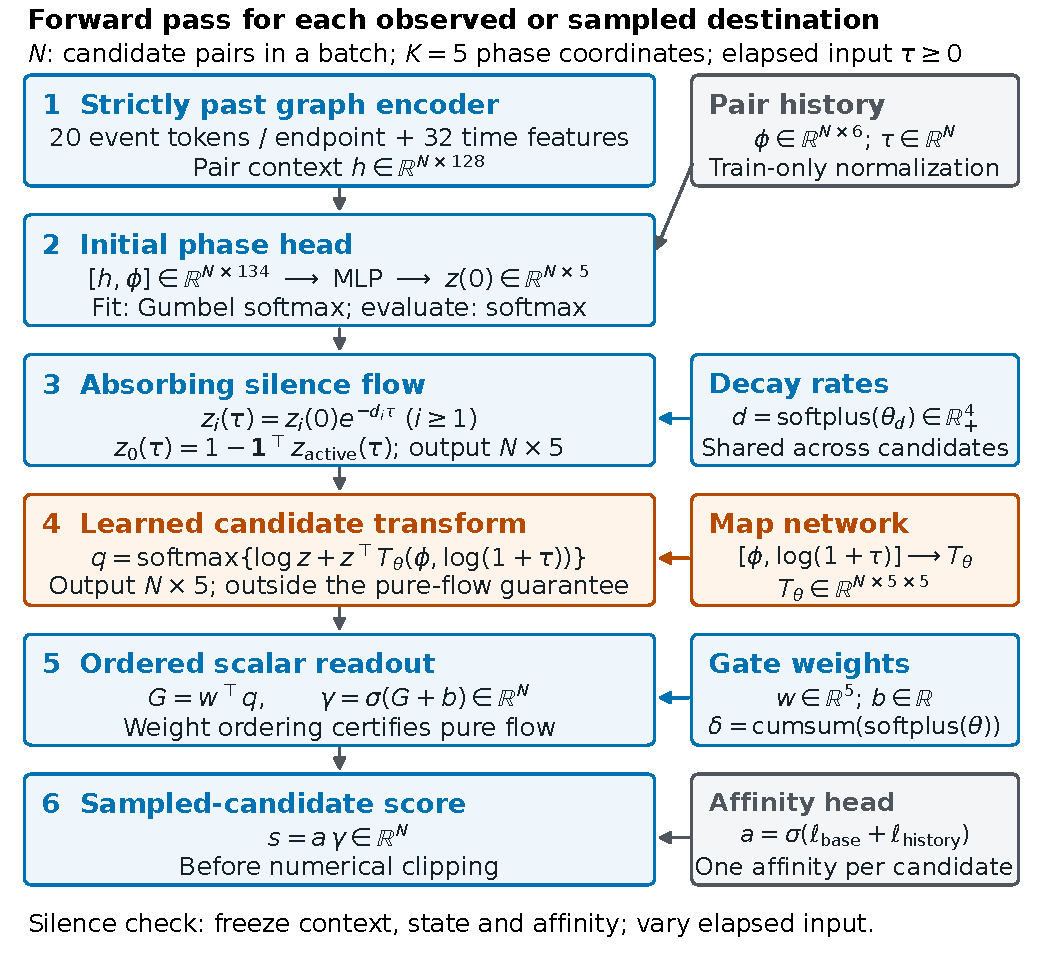
\includegraphics[width=\textwidth]{Fig1.pdf}
\caption{Tensor-level forward pipeline of the ordered Wikipedia/Reddit scorer. Dimensions are per candidate batch, with five phase coordinates and four active decay rates. The candidate network has a zero diagonal in each transition matrix and receives the historical features and explicit elapsed input. Orange boxes mark the general candidate transform outside the pure-flow guarantee; blue boxes show the state/readout path, and grey boxes supply historical context and affinity. The schematic displays the unclipped algebra; numerical guards are treated separately}\label{fig:pipeline}
\end{figure}

\section{Exact preservation and repair}\label{sec:theory}
\subsection{Pure-flow condition}
\begin{proposition}[Pure absorbing flow]\label{prop:pure}
For strictly positive active rates and fixed affinity, the untransformed readout $w^\top z(t)$ is nonincreasing for every initial simplex state if and only if $w_i\ge w_0$ for every active component. An ordering among active weights is unnecessary.
\end{proposition}
\begin{proof}
Differentiation gives
$\frac{d}{dt}w^\top z=-\sum_{i\ge1}(w_i-w_0)d_i z_i$.
Nonnegative gaps suffice. If any active gap is negative, placing all initial mass on that active component gives a positive derivative at the initial time. A strictly increasing sigmoid and a fixed positive affinity preserve this sign.
\end{proof}

Cumulative positive increments are one way of enforcing these inequalities. They are stronger than necessary when they also order active components. Conversely, unconstrained learning is not mathematically forced to violate them. Positive and negative examples contribute opposing loss gradients, so an observed inversion is a model-specific outcome.

For implementation, separate the model's forward tensors from the exact certificate inputs. Figure~\ref{fig:certificate-pipeline} shows the conversion at one fixed candidate context. Positive tilts may differ across candidates, but must stay constant along each certified elapsed-time path. At five states, four active coordinates produce six pair margins. The derivative proof augments the four-dimensional active vectors by zeros at the dormant coordinate; its auxiliary vector $a$ is distinct from the positive affinity scalar used in scoring. An automatic derivative at the observed state or a finite grid of elapsed inputs evaluates local behavior, whereas the pair condition below quantifies over every initial simplex state.
\begin{figure}[t]
\centering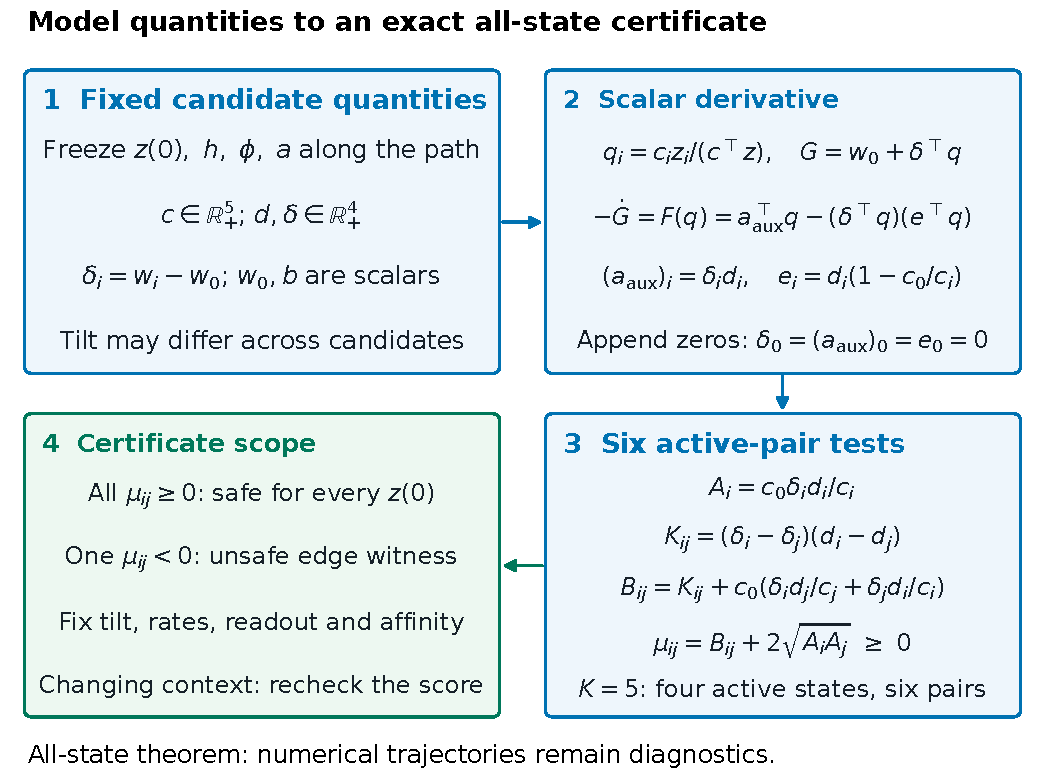
\includegraphics[width=\textwidth]{Fig2.pdf}
\caption{Bridge from frozen model quantities to the specified-rate theorem. Read panels clockwise. The diagram writes the proof's auxiliary vector as $a_{\rm aux}$ to distinguish it from the scalar affinity. Active gaps and rates may be zero, while tilts are strictly positive. All six pair margins must be nonnegative in exact arithmetic; a failed pair produces an unsafe edge-supported state. A certificate for fixed quantities does not certify a changing encoder, tilt or affinity}\label{fig:certificate-pipeline}
\end{figure}

\subsection{Specified-rate characterization}
Define
\begin{align}
A_i&=\frac{c_0\delta_i d_i}{c_i},\label{eq:A}\\
B_{ij}&=(\delta_i-\delta_j)(d_i-d_j)
+c_0\left(\frac{\delta_i d_j}{c_j}
+\frac{\delta_j d_i}{c_i}\right).\label{eq:B}
\end{align}
\begin{samepage}
\begin{theorem}[State-uniform certificate at specified rates]\label{thm:fixed}
Under \eqref{eq:flow}--\eqref{eq:tilt}, $G(t)$ is nonincreasing for every initial simplex state and every nonnegative flow time if and only if
\begin{equation}\label{eq:criterion}
B_{ij}+2\sqrt{A_iA_j}\ge0
\quad\text{for all }1\le i<j\le m.
\end{equation}
Zero gaps and zero rates are allowed. For one active component there is no pair restriction.
\end{theorem}
\end{samepage}
\begin{proof}
Set $\delta_0=a_0=e_0=0$, and for active indices let
$a_i=\delta_i d_i$ and $e_i=d_i(1-c_0/c_i)$.
Quotient differentiation yields
\begin{equation}\label{eq:F}
-\dot G=F(q)=a^\top q-(\delta^\top q)(e^\top q).
\end{equation}
Positive reweighting is a bijection of the simplex, since
$z_i=(q_i/c_i)/\sum_k(q_k/c_k)$.

For any $q$, fix $s=\delta^\top q$ and minimize $F(p)$ on
$p\ge0$, $\mathbf1^\top p=1$, $\delta^\top p=s$.
On this nonempty compact slice the objective is linear:
$F(p)=(a-se)^\top p$.
It has a minimizing extreme point supported on at most two coordinates. Indeed, more supported coordinates than the rank of the two equalities permit a nonzero supported null direction and both sufficiently small signed perturbations. If the equalities are dependent the support bound only decreases. Thus any negative margin has a witness on an edge. The two equality restrictions include normalization; the support count is not an assertion that one additional moment always gives two atoms without counting that normalization \cite{moment,pinelis}.

On an active edge with masses $u,v$ and $u+v=1$, expansion gives
\begin{equation}\label{eq:binary}
F=A_i u^2+B_{ij}uv+A_jv^2.
\end{equation}
The nonnegative diagonal terms are automatic. The standard binary criterion is \eqref{eq:criterion}, as follows from
\[
F=(\sqrt{A_i}u-\sqrt{A_j}v)^2+
(B_{ij}+2\sqrt{A_iA_j})uv.
\]
If both diagonals are positive and the criterion fails, choose $(u,v)$ proportional to $(\sqrt{A_j},\sqrt{A_i})$. If a diagonal vanishes, a sufficiently small positive mass on the other coordinate witnesses a negative value when the cross coefficient is negative; if both vanish, any interior edge mass does so. Dormant--active edges have diagonal zero at the dormant vertex and nonnegative cross coefficient $a_j$, so add no restriction. The edge reduction proves sufficiency at every state; an unsafe edge state used as an initial condition proves necessity.
\end{proof}

This support reduction is essential. Pairwise copositivity is not sufficient for a general higher-dimensional quadratic form. A matrix with unit diagonal and all off-diagonal entries $-3/4$ passes each binary test but is negative on the uniform three-vector.

To connect this argument to copositive programming, homogenize $F$ using $\mathbf1^\top q=1$:
\begin{equation}\label{eq:copositive-matrix}
F(q)=q^\top Mq,\qquad
M=\tfrac12(a\mathbf1^\top+\mathbf1a^\top
-\delta e^\top-e\delta^\top).
\end{equation}
Nonnegativity on the simplex is equivalent by scaling to copositivity of $M$ on the nonnegative orthant. This differs from positive semidefiniteness, which tests all signed directions; copositive optimization treats the former cone explicitly \cite{dur}. The binary test is classical \cite{copositive}; the useful step in this family is the reduction to two-coordinate support after fixing $\delta^\top q$. An arbitrary extra quadratic interaction can destroy that linear-on-a-slice structure, so it cannot be appended while retaining the same pair certificate.

\begin{corollary}[Rate channels and quantifier tradeoffs]\label{cor:cone}
If $d(t)=\sum_{k=1}^r\lambda_k(t)v^{(k)}$ with nonnegative finite generators and nonnegative locally integrable coefficients, the readout is nonincreasing for every such schedule and initial state if and only if \eqref{eq:criterion} holds for every generator. Necessity assumes schedules activating one generator alone are admissible.

For fixed gaps and tilt, requiring preservation for every positive rate vector is equivalent to
\begin{equation}\label{eq:allrate}
(\delta_*-\delta_i)c_i\le\delta_*c_0,\qquad
\delta_*=\max_i\delta_i.
\end{equation}
If $\delta_*=0$ the readout is constant. For a fixed rate vector, every positive constant tilt is safe if and only if
\begin{equation}\label{eq:coorder}
(\delta_i-\delta_j)(d_i-d_j)\ge0
\quad\text{for all active pairs}.
\end{equation}
\end{corollary}
\begin{proof}
The derivative at a fixed state is linear in the rate vector, which proves the cone statement and its necessity. A nonnegative exponential event dose is obtained by integrating the corresponding generator for that duration.

For the all-rate condition, make $d_i$ dominate $d_j$ in \eqref{eq:criterion}. Its leading coefficient requires
$\delta_i-\delta_j+\delta_jc_0/c_i\ge0$ for every pair. Taking the largest gap gives \eqref{eq:allrate}; when $\delta_i=0<\delta_*$ this requires $c_i\le c_0$. Sufficiency follows by checking the nonnegative orthant's unit generators, for which these inequalities are exactly the pair conditions.

Co-ordering makes the first term of every $B_{ij}$ nonnegative, proving sufficiency for arbitrary positive tilts. Conversely, for an oppositely ordered pair set both active tilts to $M$ and $c_0=1$. At equal $q$ mass on that pair, \eqref{eq:F} tends to $(\delta_i-\delta_j)(d_i-d_j)/4<0$ as $M$ grows. A finite positive tilt is therefore unsafe.
\end{proof}

The quantifiers express different modeling commitments. Specified-rate safety permits the learned rates actually being used; cone safety permits any admitted mixture or schedule of its generators; all-rate safety tolerates every nonnegative rate direction. The nesting explains why a uniform guarantee can require extra deformation. Generator coefficients need not share a clock, but must stay nonnegative. For time-varying rates the state solution uses integrated rates, $z_i(t)=z_i(0)\exp\{-\int_0^t d_i(s)\,ds\}$, and the derivative condition holds almost everywhere. State or input dependence of the tilt introduces additional derivatives absent from this statement.

The cone extension certifies exponential dose updates, not an arbitrary linear jump or reset. A changed tilt or readout restarts the scope of the statement. It does not certify an unrestricted learned transition network.

Two exact examples clarify the distinction. For $c=(1,4,4)$, $\delta=(2,1)$ and $d=(1,2)$, the pair margin is $5/4>0$. Changing the rates to $(1,10)$ makes it $-15/4+\sqrt5<0$; at $z=(0,1/2,1/2)$ the readout derivative is $3/16>0$. Figure~\ref{fig:examples}a shows both trajectories. Separately, for $c=(1,4,4)$, $\delta=d=(1,2)$ and $z=(1/10,1/10,4/5)$,
\begin{equation}\label{eq:redistribution}
\dot q_1=56/1369>0,\qquad \dot G=-1416/1369<0.
\end{equation}
Thus preserving a chosen readout need not require every active coordinate to decrease.
\begin{figure}[t]
\centering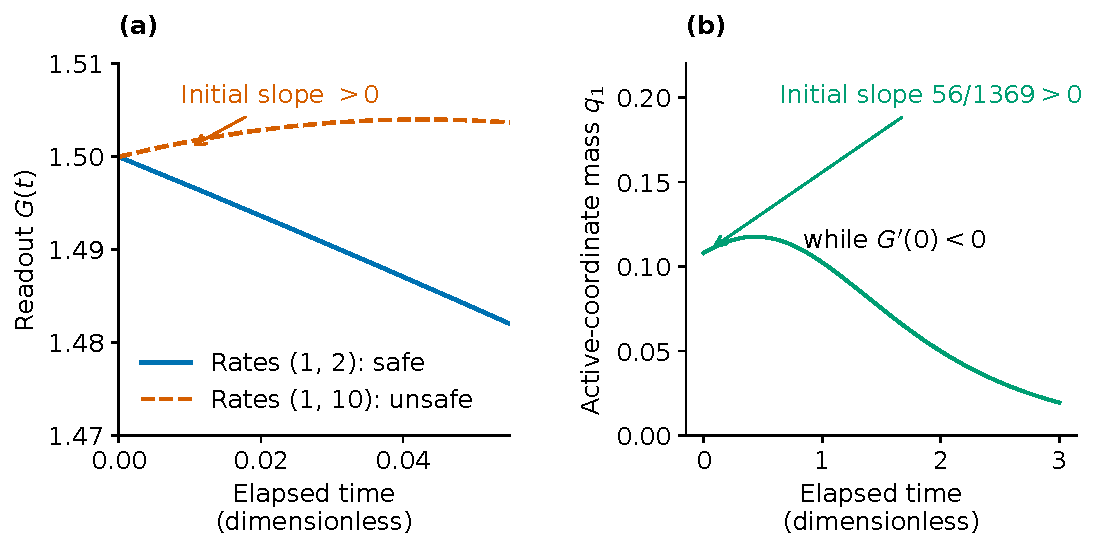
\includegraphics[width=\textwidth]{Fig3.pdf}
\caption{Exact synthetic examples, with dimensionless elapsed time. (a) A short initial-time window shows how identical tilt and readout can be safe or unsafe at different specified rates. (b) An active coordinate can initially increase while the chosen readout decreases. Parameters and initial slopes are given in the text; these are mathematical examples, not fitted relationship lifetimes}\label{fig:examples}
\end{figure}

\subsection{Halfspace geometry and a matched repair}
Let $x_i=\sqrt{c_0/c_i}>0$ and $K_{ij}=(\delta_i-\delta_j)(d_i-d_j)$. Direct factorization gives
\begin{equation}\label{eq:factor}
B_{ij}+2\sqrt{A_iA_j}
=K_{ij}+
\left(\sqrt{\delta_jd_i}\,x_i+
\sqrt{\delta_id_j}\,x_j\right)^2.
\end{equation}
Pairs with $K_{ij}\ge0$ are automatically safe. Otherwise the exact condition is the halfspace
\begin{equation}\label{eq:halfspace}
\sqrt{\delta_jd_i}\,x_i+
\sqrt{\delta_id_j}\,x_j\ge\sqrt{-K_{ij}}.
\end{equation}
For a finite rate cone the rows are stacked over its generators, yielding $Hx\ge h$, with $H\ge0$ and at most $O(rm^2)$ rows.

\begin{theorem}[Projection in inverse-tilt coordinates]\label{thm:projection}
For $x^0>0$, the problem
\begin{equation}\label{eq:projection}
\min_{x\ge0,\ Hx\ge h}\frac12\|x-x^0\|_2^2
\end{equation}
has a unique minimizer $x^*$ with $x^*\ge x^0>0$. It therefore solves the positive-tilt problem without an arbitrary positivity floor.
\end{theorem}
\begin{proof}
Every nonzero row of $H$ has a positive coefficient, so a sufficiently large positive constant vector is feasible. The closed feasible set is nonempty, and the objective is coercive and strictly convex. If a coordinate of the minimizer were below its value in $x^0$, increasing it to that value would strictly improve the objective and could not hurt a nonnegative lower constraint. Hence $x^*\ge x^0$.
\end{proof}

The dual has $\lambda\ge0$, $x=x^0+H^\top\lambda$ and
\[
D(\lambda)=\lambda^\top(h-Hx^0)
-\tfrac12\|H^\top\lambda\|_2^2.
\]
A standard coordinate update is
$\lambda_j\leftarrow\max\{0,\lambda_j+(h_j-H_jx)/\|H_j\|^2\}$.
We normalize nonzero rows and check primal feasibility, dual feasibility, stationarity and complementarity. A fixed numerical budget may fail; such a failure is not reported as a certified optimum.

This construction separates finding a feasible point from finding the nearest one in a declared metric, a distinction central to projection methods \cite{projection,dykstra}. The chosen halfspaces and strictly convex quadratic give a unique primal answer even if redundant rows make the dual multipliers nonunique. For nonempty constraint rows, a sufficiently large positive $x$ satisfies every inequality strictly; standard convex duality therefore applies \cite{convex}. The lower bounds $x\ge0$ may be omitted from the dual calculation because the halfspace-only projection already obeys $x\ge x^0>0$ by the same coordinate-increase argument.

For a feasible primal iterate $x$ and any $\lambda\ge0$, let $P(x)=\tfrac12\|x-x^0\|_2^2$. Weak duality and strong convexity provide a useful accuracy interpretation:
\begin{equation}\label{eq:gap-bound}
0\le P(x)-P(x^*)\le P(x)-D(\lambda),\qquad
\|x-x^*\|_2\le\sqrt{2\{P(x)-D(\lambda)\}}.
\end{equation}
The distance bound requires primal feasibility; a small stationarity residual alone is insufficient. These are exact-arithmetic optimization statements. Floating-point residuals and tolerances remain numerical diagnostics, and no ranking-optimality claim follows.

For comparison, \eqref{eq:allrate} becomes
$x_i\ge\sqrt{(\delta_*-\delta_i)/\delta_*}$ when $\delta_*>0$.
Its Euclidean projection is coordinatewise clipping to these lower limits. Because its feasible set is a subset of the specified-rate set,
\begin{equation}\label{eq:distance}
\|x^{\rm specified}-x^0\|_2^2
\le\|x^{\rm all}-x^0\|_2^2.
\end{equation}
This is a same-metric distance statement, not an ordering of AP or prediction error. Figure~\ref{fig:geometry} illustrates a nontrivial synthetic projection. For $\delta=(2,1)$ and $d=(1,2)$, the exact halfspace is $x_1+2x_2\ge1$. The projection of $(1/10,1/10)$ is $(6/25,19/50)$.
\begin{figure}[t]
\centering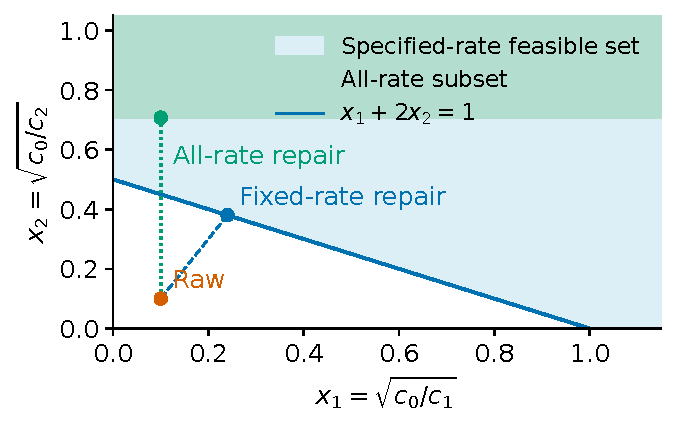
\includegraphics[width=.74\textwidth]{Fig4.pdf}
\caption{Exact feasible geometry in a two-active-component example. The specified-rate region includes the stronger all-rate region. Both repairs minimize the same Euclidean distance in $x$ coordinates. The illustrated nontrivial repair is synthetic; the retained real-model specified-rate points below are already feasible}\label{fig:geometry}
\end{figure}

\section{Empirical design}\label{sec:design}
\subsection{Distinct questions and populations}
We use three complementary studies. The first compares independently fitted prediction variants on shared historical negatives in Wikipedia and Reddit. The second is a post hoc fixed-context path analysis and no-refit repair comparison on the retained ordered models' supported validation queries. The third tests a same-information phase residual on original Last.fm listening histories, followed by a fixed next-month check. Their populations, selection histories and endpoints differ. We do not pool their AP values or use the repair study as a new predictive test.

Wikipedia and Reddit are the interaction datasets distributed with the JODIE study \cite{jodie}. We retain 157,474 and 672,447 events respectively, construct disjoint user/item namespaces, and use chronological 70/15/15 percent splits. Ten percent of test-incident nodes are sampled for training exclusion using split seed 42. Events incident to these held-out nodes enter neither training supervision nor training history. Other allowed events without a supported candidate still enter history.

For an observed destination and a historical negative from the same source, let $c$ be the strictly prior pair count and $\tau$ the time since its latest event. The negative must have prior history and satisfy the same bins
\begin{equation}\label{eq:matching}
b_c=\lfloor\log_2 c\rfloor,\qquad
b_\tau=\left\lfloor\log_2(1+\tau/u)\right\rfloor,
\end{equation}
where $u=1000$ seconds for Wikipedia/Reddit. All simultaneous observed destinations are forbidden negatives. Every timestamp group is queried before any member updates history. If the eligible pool is empty, supervision is omitted without an easier fallback. Matching bins does not make raw counts or times identical. Table~\ref{tab:coverage} reports the resulting conditional support.

\begin{table}[t]
\caption{Conditional support under shared history-bin matching.}\label{tab:coverage}
\centering
\begin{tabular}{@{}lrrrrr@{}}
\toprule
Dataset & Train & Validation & Test & Unsupported & Excluded \\
\midrule
Wikipedia & 2,805 & 884 & 977 & 138,000 & 14,808 \\
Reddit & 37,206 & 10,139 & 11,002 & 538,695 & 75,405 \\
\botrule
\end{tabular}
\begin{tablenotes}[flushleft]\footnotesize\item Counts are queries or events, not candidate trajectories. Each supported query has one positive and one negative. Support counts agree across seeds. Unsupported events are omitted from supervision; training-excluded events enter neither training supervision nor training history. Totals are 157,474 Wikipedia and 672,447 Reddit events.\end{tablenotes}
\end{table}

\subsection{Common encoder and prediction controls}
The encoder aggregates the last 20 strictly earlier events of each endpoint. Event features are concatenated with a 32-dimensional sinusoidal time representation and projected to width 128. A token-mixing multilayer perceptron (MLP) and a channel-mixing MLP with layer normalization process each endpoint history; masked averaging gives endpoint vectors. Their concatenation, absolute difference and elementwise product feed a pair projection and affinity scorer. This is a common encoder, not a reproduction of an official benchmark architecture.

Five prediction variants are fitted independently: neighbor affinity; affinity with explicit history; an exponential scalar gate with history; a flexible sigmoid MLP gate with history; and a five-component ordered phase gate with history. The six history channels are a smoothed exponential recency statistic, $\log(1+\tau)$, $\log(1+c)$, prefix-normalized count, and sine/cosine time of day. Their normalizers use training candidates only. The recency statistic is $0.1+0.9e^{-0.01\tau}$ and the prefix count is $c/\sqrt{\max(1,n)}$, with $n$ the preceding-event index.

All variants use Adam, learning rate $10^{-3}$, weight decay $10^{-5}$, ten epochs and batch size 256. Seeds are 1, 7 and 42, with common backbone initialization and minibatch ordering within a seed. The earliest maximum-validation-AP epoch selects the model evaluated on the test split. Decay inputs use a fixed 1000-second scale. Task and affinity auxiliary supervision are shared, while the phase variant additionally uses entropy, diversity and transition-sparsity penalties. Parameter counts and regularization differ: the comparison controls information access and evaluation, not every effect of capacity or objective.

The phase encoder maps the pair representation and history to a simplex state, using Gumbel softmax during fitting and deterministic softmax during evaluation. Its candidate transform has the form
\begin{equation}\label{eq:learnedmap}
q=\operatorname{softmax}\{\log z+\ z^\top T_\theta(\phi,\log(1+\tau))\}.
\end{equation}
The active readout weights exceed the dormant weight through cumulative softplus increments. Equation~\eqref{eq:learnedmap} is evaluated for both candidates before the event is observed; it is a scoring transform, not an observed post-interaction update.

\subsection{Learned-path analysis and no-refit repair}
For every supported validation query of the ordered Wikipedia and Reddit models, we hold native encoder outputs, initial state and affinity fixed. We evaluate a 25-point logarithmic grid of normalized elapsed inputs from $10^{-3}$ to $10^3$. A trajectory is flagged if an adjacent unclipped native-float32 score increases by more than $10^{-5}$. We retain ideal flow, implemented flow, a frozen transition matrix and the explicitly time-dependent transition path. The frozen matrix is evaluated at the observed anchor, but its product with the flowing state still changes.

Coverage expansion was fixed after an earlier anchor diagnostic; it is a post hoc characterization, not independent confirmation. Numerical threshold non-crossing is not an exact monotonicity proof. The diagnostic reconstructs all retained query contexts, and compares native and float64 path scores and derivatives. It does not retrain the models or recompute their encoders over artificial future histories.

The repair comparison first freezes the learned transition at zero reference clock, then projects that matrix onto $T_{ij}=\beta_j-\beta_i$. Here $\beta$ denotes a potential vector, distinct from the scalar gate bias $b$. For this gradient form,
$z^\top T$ equals $\beta$ up to a common additive shift, so \eqref{eq:learnedmap} reduces to \eqref{eq:tilt} with $c_i=e^{\beta_i}$. The least-squares potential is
$\widehat\beta_j=(\sum_iT_{ij}-\sum_iT_{ji})/[2(m+1)]$, followed by the gauge $\widehat\beta_0=0$.
This operation has already changed the original scorer. We compare specified-rate and all-rate repairs in the same $x$ metric, retaining the unconstrained gradient comparator and original dynamic score as separate references. Primary repair scoring uses a float64 lift of archived native parameters and reference potentials.

Figure~\ref{fig:repair-pipeline} separates these operations for a practitioner applying the theorem to a trained network. Freezing the clock removes explicit time dependence in $T$ but leaves the product $z^\top T$ state dependent. The gradient-form fit is the additional restriction that makes the normalized tilt constant. Only after those two reference changes do the two inverse-tilt repairs share the same initial point and metric. Each repaired point is converted back to a potential and rescored with common initial state, decay rates, weights and affinity. The original dynamic predictor remains a separate comparator; this workflow does not retrofit a guarantee to its unrestricted computation.
\begin{figure}[t]
\centering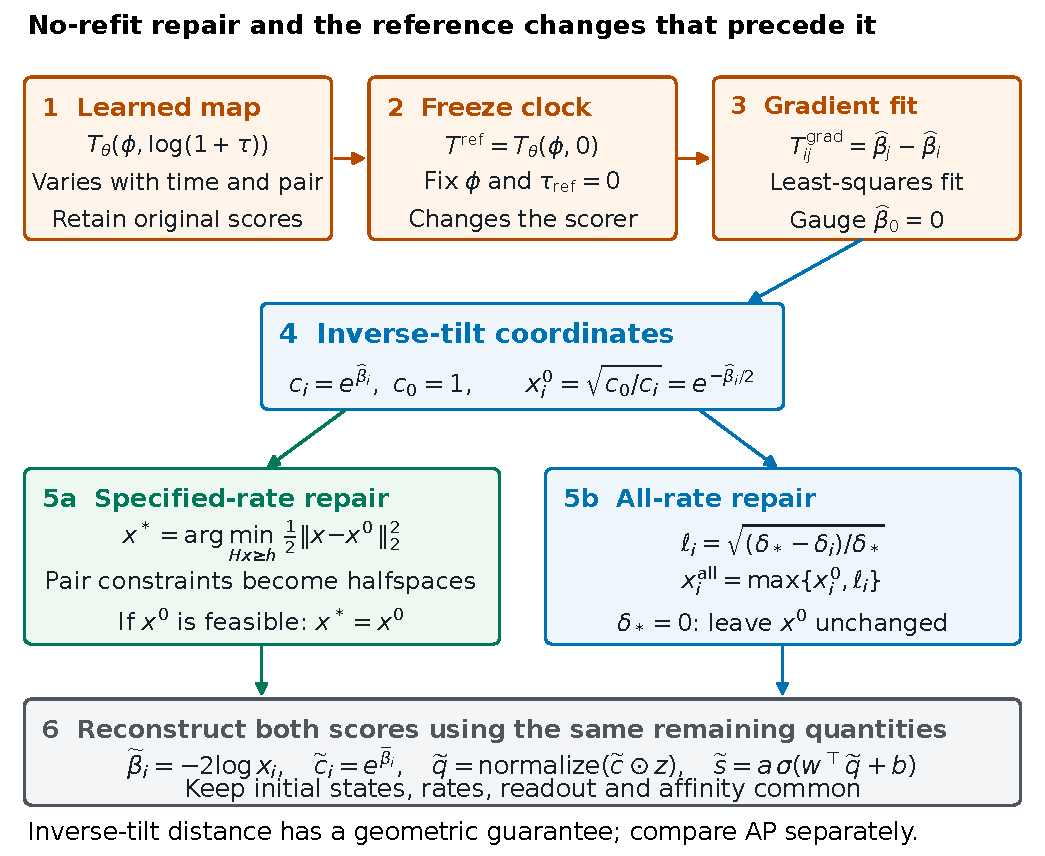
\includegraphics[width=\textwidth]{Fig5.pdf}
\caption{No-refit application of the theorem to retained neural scorers. The first three stages distinguish the original candidate map, its frozen reference and a gradient-form matrix approximation. The gauge makes $c_0=1$. Both repair branches use Euclidean distance in the same inverse-tilt coordinates; the specified-rate branch uses halfspaces, while the all-rate branch clips to coordinate lower bounds. For the latter, $\delta_*=\max_i\delta_i$ and its displayed formula assumes $\delta_*>0$. Reconstruction keeps the dormant potential zero. Geometric minimality and AP are assessed separately}\label{fig:repair-pipeline}
\end{figure}

\subsection{Listening-history follow-up}
Original Last.fm-1K listening histories are obtained from the creator-attributed data release \cite{lastfm,celma}, originally collected from Last.fm (\url{https://www.last.fm/}). A fixed hash ranking with seed 17 selects 100 profile IDs; inactive IDs are not replaced. The training history contains 1,762,318 events before 1 January 2009. January provides development validation; February is the subsequent held-out evaluation. Missing-track events remain in source activity and neighborhoods but do not create a shared artificial item. Training query selection retains one sixteenth of hash-selected eligible queries while preserving the complete event history. All supported later queries are retained.

Only recurrent user--track queries with at least one hour since their previous event are eligible. Historical negatives use \eqref{eq:matching} with $u=3600$ seconds. The latest strictly prior own-track timestamp group determines a frozen artist reference, with missing/conflicting reference groups flagged. The dose $E$ counts strictly intervening events having that recorded artist. The current event's metadata cannot enter its own reference. Training-known artists use a 32-dimensional embedding; later new artists retain the unknown lookup. Typed user/item graph neighborhoods prevent numeric-ID collisions.

Six arms share the encoder and eleven history channels: history-only, a flexible time/dose residual, a proportional-rate clock residual, an independent-rate phase residual, an alternate-reference phase residual and an activity-only residual. The phase and flexible primary branches each have 13 additional parameters. The alternate artist is drawn deterministically from a different artist already observed at the reference time and then frozen. This is not a marginal-preserving causal randomization. The activity arm masks the same-artist channel in both head and branch, while graph history can still contain artist information.

Every own group resets the phase state to uniform over five components. The readable phase residual is
\begin{equation}\label{eq:residual}
r(\tau,E)=\sum_{j=1}^4 b_j
\{\exp(-k_j\tau-h_jE)-1\},\qquad b_j\ge0,\ k_j,h_j>0.
\end{equation}
Its coefficients and rate units are determined by training. The full logit is the jointly trained base logit plus $r$. A proportional control uses event rates proportional to physical-time rates; a two-input, three-hidden-unit GELU MLP supplies the flexible control. Adam settings and the ten-epoch budget match the earlier optimizer settings, with batch size 512 and affinity auxiliary weight $0.5$. Seeds are 101, 202 and 303. Checkpoints are selected by earliest maximum January AP.

An exploratory January partition used three gap and three dose bins, retaining all marginals and intersections. The chosen follow-up population has positive-query gap $[1,7)$ days and same-artist dose $[1,10)$. February preparation and scoring occurred only after fixing that population, all eighteen selected checkpoints, candidate rules and the endpoint. Neither fitting nor checkpoint reselection occurs in February. Both candidates of every selected query remain in the cohort; this is a retrospective label-defined population, not a deployable candidate filter.

The February endpoint is the mean of the three seed-paired phase-minus-flexible AP differences. Support requires at least 100 primary queries and ten active users at every seed. A paired positive-user-cluster bootstrap samples the retained active primary users with replacement, assigning each user's multiplicity to both candidates in every seed pair. We use 2000 replicates, PCG64 seed 20261016, and linear 2.5/97.5 percentile quantiles. The local screen requires support, positive differences at every seed and a positive lower interval endpoint. Other cohorts or metrics cannot replace it.

\subsection{Metrics and verification}
AP is computed over the pooled positive and matched-negative scores within the specified population, with each query contributing one of each. We also retain area under the receiver operating characteristic curve (AUC) and pair accuracy, giving ties half credit for pair accuracy. Across-seed standard deviations are descriptive variation across fitted model/candidate seeds, not population confidence intervals. The user-cluster interval is conditional on frozen models and February; it excludes optimizer uncertainty, other months and cross-user graph dependence.

Retained checkpoints are replayed independently on a central processing unit (CPU), and score-derived metrics are reconstructed using tie-aware rank calculations. The theoretical identities and witnesses are checked with exact algebra; synthetic quadratic-program (QP) solutions are compared with exhaustive small active-set solutions. Numerical Karush--Kuhn--Tucker (KKT) checks support the implemented solver but are not formal floating-point proofs. The fitted environment reports Python 3.13.15, PyTorch 2.11.0 with CUDA 13.0, and NumPy 2.1.3. All figures were prepared with Matplotlib and exported as vector PDF/EPS artwork. Dependency ranges were bounded rather than fully locked; inference agreement does not imply reproducibility of the complete optimization trajectory in a fresh environment.

\section{Results}\label{sec:results}
\subsection{An intermediate guarantee does not certify the scored path}
Table~\ref{tab:paths} and Fig.~\ref{fig:paths} report every retained dataset/seed. Each Wikipedia seed covers 884 validation queries, hence 1768 candidate trajectories; each Reddit seed covers 10,139 queries, hence 20,278 trajectories. In total there are 66,138 model-candidate trajectories across six cohorts. These are repeated queries across model seeds, not independent relationship lifetimes.

\begin{table}[t]
\caption{Native-score path violations on supported validation candidates.}\label{tab:paths}
\centering
\begin{tabular}{@{}llrrrr@{}}
\toprule
Dataset & Seed & Candidates & Flow & Frozen map & Dynamic map \\
\midrule
Wikipedia & 1 & 1,768 & 0 & 0 & 0 \\
Wikipedia & 7 & 1,768 & 0 & 0 & 0 \\
Wikipedia & 42 & 1,768 & 0 & 0 & 0 \\
Reddit & 1 & 20,278 & 0 & 18,037 & 20,075 \\
Reddit & 7 & 20,278 & 0 & 14,102 & 20,270 \\
Reddit & 42 & 20,278 & 0 & 15,042 & 20,278 \\
\botrule
\end{tabular}
\begin{tablenotes}[flushleft]\footnotesize\item Entries are counts of trajectories with at least one adjacent increase above the declared threshold. Candidates count both destinations for every supported query. All six dataset/seed cohorts are retained.\end{tablenotes}
\end{table}

None of the pure implemented-flow paths crosses the declared threshold. The complete Reddit paths do so on 98.9989--100 percent of trajectories, whereas the complete Wikipedia paths have no crossing. Even the frozen Reddit transition matrix permits many reversals because the state entering $z^\top T$ changes. The observation is therefore more specific than a claim that explicit transition-time drift alone causes the problem.

All native and float64 dynamic-path violation flags agree. One secondary frozen-map flag differs near the threshold, so the prespecified native result is retained. The largest pointwise native/float64 discrepancy is below $6.5\times10^{-7}$. These results delimit the measured scorer paths; they do not prove that every trained map violates a certificate or that zero observed flags imply an all-time guarantee.
\begin{figure}[t]
\centering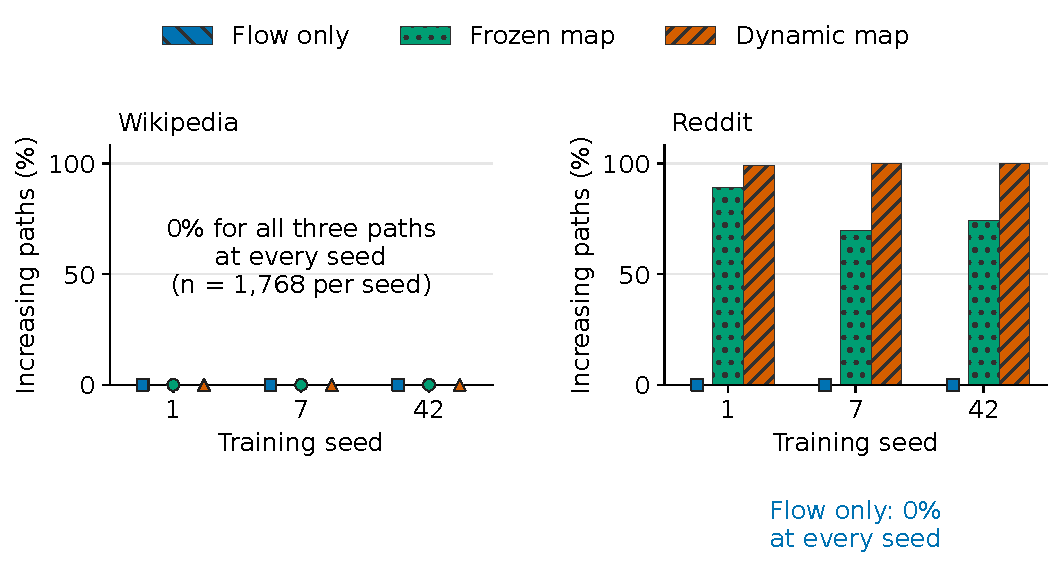
\includegraphics[width=\textwidth]{Fig6.pdf}
\caption{Complete supported-validation path diagnostics. A violation means an adjacent unclipped score increase above $10^{-5}$ on the fixed 25-point grid. Encoder context and affinity stay fixed. Zero-valued observations are explicitly marked on the baseline. Zero observed Wikipedia flags are threshold non-crossings, not mathematical proofs; the high Reddit fractions concern retained model paths, not physical relationship trajectories}\label{fig:paths}
\end{figure}

\subsection{Sharper certification avoids extra deformation}
Every frozen-reference gradient comparator passes the specified-rate certificate, with minimum pair margin $0.1730612789$ across all 66,138 candidate configurations. Specified-rate projection therefore leaves every raw $x$ unchanged. In contrast, the all-rate repair changes 46,619 Reddit candidate configurations and no Wikipedia configurations. Figure~\ref{fig:repair} retains the individual seeds. The real specified-rate optimizations require no coordinate updates; their outcome is a certification result, while nontrivial optimization is checked synthetically.

\begin{table}[t]
\caption{Same-metric no-refit repair comparison on validation queries.}\label{tab:repair}
\centering
\begin{tabular}{@{}llrrrr@{}}
\toprule
Dataset & Seed & Specified AP & All-rate AP & $10^6\Delta$AP & Changed \\
\midrule
Wikipedia & 1 & 0.5715580 & 0.5715580 & +0.0000 & 0 \\
Wikipedia & 7 & 0.5673776 & 0.5673776 & +0.0000 & 0 \\
Wikipedia & 42 & 0.5738074 & 0.5738074 & +0.0000 & 0 \\
Reddit & 1 & 0.5242809 & 0.5242823 & -1.3959 & 16,474 \\
Reddit & 7 & 0.5264003 & 0.5264002 & +0.0397 & 19,193 \\
Reddit & 42 & 0.5270709 & 0.5270732 & -2.3466 & 10,952 \\
\botrule
\end{tabular}
\begin{tablenotes}[flushleft]\footnotesize\item $\Delta$AP is specified-rate minus all-rate AP; its scale is shown explicitly because differences are small. Changed counts refer to the all-rate repair; the specified-rate repair changes zero candidates in every row. The mean Reddit difference is $-1.2343\times10^{-6}$ (sample SD $1.2013\times10^{-6}$).\end{tablenotes}
\end{table}

The primary AP comparison does not show a mean predictive advantage. Specified-rate AP is identical to its raw gradient comparator at every seed. Relative to the original dynamic scorer, the mean AP difference remains approximately $-0.000135934$ on Wikipedia and $-0.027708126$ on Reddit. Much of the ranking change therefore precedes the final certificate, when the original map is converted to the restricted reference family. The geometric guarantee in \eqref{eq:distance} must not be restated as a ranking guarantee. Precision--recall and ROC criteria measure different aspects of a ranking \cite{prroc}; neither is the quadratic objective in \eqref{eq:projection}. For distinct scores, AP averages the precision at positive ranks. A small candidate-dependent perturbation can swap a nearly tied positive and negative, changing AP, whereas a common strictly increasing transformation preserves all ranks. Minimizing tilt distance is neither of these ranking conditions. Any implication for AP would require further score-separation or ranking analysis.
\begin{figure}[t]
\centering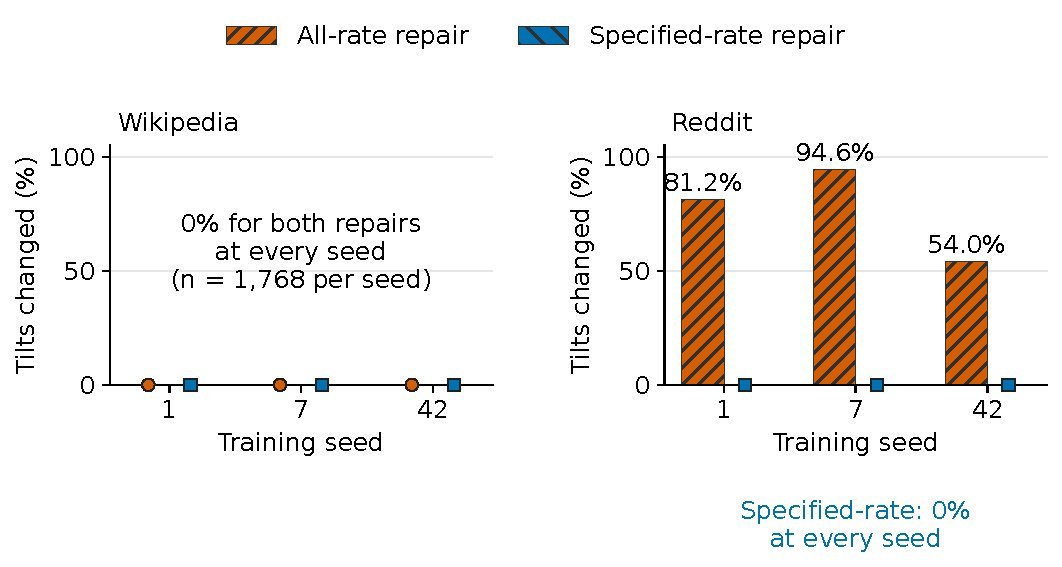
\includegraphics[width=\textwidth]{Fig7.pdf}
\caption{Additional deformation of the frozen-reference gradient comparator. The all-rate restriction changes many Reddit tilts, while the specified-rate certificate accepts all retained raw points. Zero-valued observations are explicitly marked on the baseline. The original dynamic predictor was already changed to obtain this comparator; zero additional deformation does not mean preservation of the original predictor}\label{fig:repair}
\end{figure}

\subsection{Matched-history predictive effects are mixed}
Table~\ref{tab:prediction} presents the original pooled test AP endpoint. On Wikipedia the ordered gate is below both the history-aware baseline and flexible gate. On Reddit it has a modest mean advantage over the history-aware baseline at every seed, but beats the flexible gate at only two of three seeds. Because capacity and regularization also differ, these outcomes compare implemented variants rather than isolating the readout constraint alone.

\begin{table}[t]
\caption{Pooled test AP with common history-matched negatives.}\label{tab:prediction}
\centering
\begin{tabular}{@{}lcc@{}}
\toprule
Prediction variant & Wikipedia & Reddit \\
\midrule
Neighbor affinity & $0.59892\pm0.01269$ & $0.53860\pm0.00057$ \\
Affinity + history & $0.61148\pm0.01111$ & $0.54764\pm0.00123$ \\
Scalar gate + history & $0.54281\pm0.00572$ & $0.51281\pm0.00352$ \\
Flexible gate + history & $0.61348\pm0.01645$ & $0.54808\pm0.00341$ \\
Ordered phase gate + history & $0.56335\pm0.00473$ & $0.54979\pm0.00019$ \\
\botrule
\end{tabular}
\begin{tablenotes}[flushleft]\footnotesize\item Mean and sample SD over seeds 1, 7 and 42. Test support is 977 queries per Wikipedia seed and 11,002 per Reddit seed. These are conditional internal-architecture comparisons; the values are not comparable with easier-negative benchmark tables.\end{tablenotes}
\end{table}

The contrast between Tables~\ref{tab:paths} and \ref{tab:prediction} is substantive. The retained Reddit model can show a modest predictive gain while failing the artificial scored-path silence test, whereas the Wikipedia model can lose AP without threshold crossings in that diagnostic. Neither structural compliance nor noncompliance determines predictive utility by itself.

\subsection{The localized listening-history gain does not pass February confirmation}
January development AP is reported in Table~\ref{tab:lastfm}. The phase-minus-flexible mean is $-0.000078712$, with mixed seed signs. The phase arm is below history-only at all three seeds. Thus the aggregate comparison does not support a new phase-based predictor advantage.

\begin{table}[t]
\caption{January Last.fm development comparison.}\label{tab:lastfm}
\centering
\begin{tabular}{@{}lrc@{}}
\toprule
Prediction variant & Branch parameters & AP \\
\midrule
History only & 0 & $0.720691\pm0.001200$ \\
Flexible time/dose residual & 13 & $0.720405\pm0.001147$ \\
Proportional-rate clock & 10 & $0.720443\pm0.000816$ \\
Independent-rate phase & 13 & $0.720326\pm0.000969$ \\
Alternate-reference phase & 13 & $0.720380\pm0.000379$ \\
Activity-only residual & 13 & $0.720243\pm0.000414$ \\
\botrule
\end{tabular}
\begin{tablenotes}[flushleft]\footnotesize\item Mean and sample SD over seeds 101, 202 and 303; 40,600 validation queries per seed. Every arm uses the same 1,054,378-parameter history backbone. Phase versus flexible residual is the primary same-input, equal-branch-parameter contrast. These are checkpoint-selection-window outcomes.\end{tablenotes}
\end{table}

The exploratory positive-query subgroup with gap $[1,7)$ days and dose $[1,10)$ has 4210 January queries from 58 users. Its phase-minus-flexible mean is $+0.001030066$ and all three seed differences are positive. The subsequent fixed February subgroup contains 4328 queries from 57 users; its seed differences are $-0.000303788$, $+0.000487551$ and $+0.000085794$. The mean is $+0.000089853$, with conditional bootstrap interval $[-0.001374495,+0.001248376]$. One seed loses and the lower endpoint is negative, so the declared local screen fails. Figure~\ref{fig:holdout} shows the discovery and follow-up together.

This outcome neither proves equality nor rules out every possible benefit. It prevents promotion of the observed January localization into a confirmed operating-region claim. All six arms, sixteen cohorts and five contrasts remain retained; no secondary significance search replaces the primary. February has been used and is not an untouched evaluation window for later designs. Across the entire February population the phase-minus-flexible mean is $-0.000060712$.
\begin{figure}[t]
\centering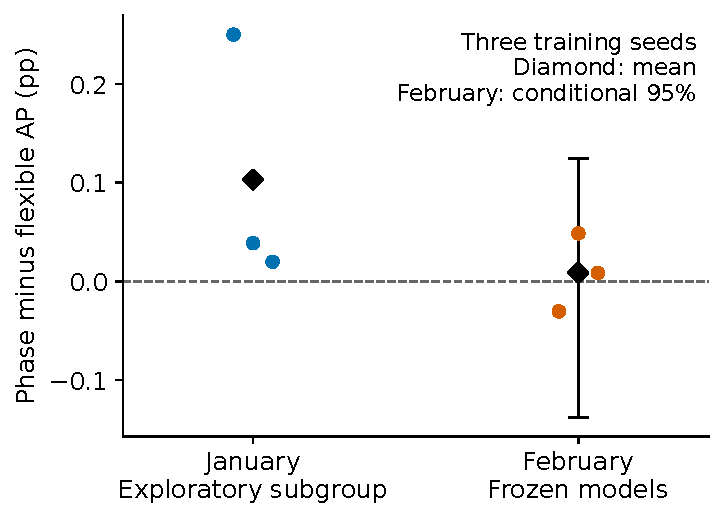
\includegraphics[width=.82\textwidth]{Fig8.pdf}
\caption{The exploratory January subgroup and the fixed February follow-up. Points show individual model-seed AP differences and diamonds their means. The February error bar is the conditional percentile interval from paired user-cluster resampling, not a training-seed or population interval. The fixed local-confirmation screen is not met}\label{fig:holdout}
\end{figure}

\section{Interpretation and limitations}\label{sec:discussion}
\subsection{What the mathematical result establishes}
The certificate gives a finite decision procedure, an unsafe edge witness when the condition fails, and a convex repair in explicit coordinates for the declared absorbing family. It separates the rates actually specified from the stronger demand to tolerate every positive rate vector. A readout-specific requirement also permits redistribution among active coordinates. These statements can guide a model designer without assigning any semantic lifecycle name to those coordinates.

Their domain is restrictive. Tilts, readout, initial-state construction, affinity and context must remain fixed along the certified path. A learned state-dependent candidate map or changing temporal encoder is outside that theorem. Converting a learned transition into a constant-tilt gradient form changes the model before projection. The small Euclidean repair distance is measured in inverse-tilt coordinates and need not correspond to a small change in probability, ranking or scientific interpretation.

The mathematical ingredients are known, and the result is positioned as a specialized characterization. The source comparison establishes differences from inspected sufficient predicates, not priority against every equivalent formulation. Exact symbolic checks and finite optimizer tests are also distinct from external proof review or a formal proof-assistant verification.

\subsection{Explanation of a branch and explanation of a predictor}
Intrinsic interpretability and a post hoc account of a black-box predictor are distinct aims \cite{rudin}. Normalized internal weights also require an explicit explanation target: Jain and Wallace show that attention weights can vary without equivalent explanatory changes in the studied NLP systems \cite{attention}, while Wiegreffe and Pinter emphasize model-aware tests and the dependence on what counts as an explanation \cite{attentiontests}. These are precedents about the interpretation of internal weights, not experiments on our temporal graph model. Here we ask the narrower, verifiable question of how a declared branch contributes to a fixed prediction.
Equation~\eqref{eq:residual} exposes the phase branch's additive contribution to a logit. If $B=\sum_j b_j$, then
\begin{equation}\label{eq:influence}
-B\le r(\tau,E)\le0,\qquad
0\le\sigma(\ell_{\rm base})-\sigma(\ell_{\rm base}+r)\le B/4.
\end{equation}
The probability bound uses the sigmoid's maximum derivative $1/4$. It is a fixed-base influence bound, not an AP bound or a bound on the branch's influence during joint fitting.

Across all retained January phase predictions, component sums reconstruct the branch and base-plus-branch reconstructs the final logit. The mean direct probability reduction is only 0.042--0.087 percentage points across the three seeds. This is a faithful account of a small constrained component, while the dominant base scorer remains opaque. Simultaneously permuting component rates and coefficients leaves the branch unchanged, so component indices do not identify lifecycle stages. Physical-time and dose effects interact inside each exponential; a unique additive causal allocation between them does not follow.

\subsection{Statistical and operational scope}
Historical matching narrows the estimable population. Unsupported first-time pairs and queries with no eligible historical negative are not evaluated by these conditional endpoints. Counts and elapsed times are only matched by bins, and score comparability across queries remains relevant to pooled AP. A weak result under this distribution does not imply a weak result under every deployment candidate distribution.

The experiments use fixed, limited budgets and internal architectures, not an exhaustive hyperparameter search or a matched comparison with every contemporary temporal model. Model-seed variation does not estimate user-population uncertainty. The February interval conditions on the selected models, active users and observed month and excludes cross-user graph dependence. The data contain recorded interactions and identity proxies, not measured relationship termination, causal displacement or verified latent stages.

The no-refit comparisons and path diagnostics are retrospective on retained checkpoints. The February design is prospective relative to preparation/scoring of that month, but follows January subgroup discovery in the same sampled listening population. These distinctions constrain the strongest supported statement: the specified architectural property can be checked, yet it does not establish a reliable predictive advantage or a comprehensive explanation of the complete model.

\section{Conclusion}
We characterize preservation of a fixed readout under positive reweighting of an absorbing simplex flow at specified rates, extend the condition to admissible rate channels, and expose an exact halfspace repair in inverse-tilt coordinates. The characterization distinguishes readout preservation from coordinatewise decline and from a guarantee uniform over all rates. Complete retained-model diagnostics and controlled prediction comparisons show why these distinctions matter operationally. Sharper certification avoids unnecessary additional deformation within its restricted comparator family, while predictive gains remain mixed or unconfirmed. A useful monotone temporal component therefore requires both an explicit certificate domain and evaluation that controls information access, candidate support and selection history.

\section*{Statements and Declarations}
\subsection*{Funding}
The authors received no funding for this work.
\subsection*{Competing interests}
The authors declare no competing interests.
\subsection*{Ethics approval and consent}
This study performs secondary analysis of publicly released historical interaction datasets. It did not recruit participants, collect new personal data or conduct interventions on individuals. No study-specific ethics approval was obtained. No identifying participant images or personal case descriptions are included. Consent to participate and consent for publication are not applicable to the secondary analysis reported here.
\subsection*{Data availability}
Wikipedia and Reddit interaction records are available from the original SNAP/JODIE providers \cite{jodie}. The original Last.fm-1K release is available from its creator-attributed repository \cite{lastfm}. Source data remain subject to the providers' terms and are not redistributed here. Aggregate data used in the figures and the complete reported comparison tables accompany the manuscript.
\subsection*{Code availability}
The research implementation, study configurations, implementation tests and figure generators are available at \url{https://github.com/hoangduong6210/lifecycle-readout}. The manuscript supplies the mathematical definitions, proof details, optimization updates and aggregate figure data. Trained model checkpoints and local run archives are not distributed.
\begin{appendices}
\section{Spectral-ratio boundary examples}\label{app:spectral}
For distinct positive active rates and positive initial active masses, the denominator coefficients in \eqref{eq:spectral} are $\beta_0=c_0$ and $\beta_i=(c_i-c_0)p_i$. If all active tilts exceed $c_0$, the corresponding numerator/denominator coefficient quotients are $0$ and $\delta_i c_i/(c_i-c_0)$. For
\[
c=(1,2,11/10,2,11/10),\qquad \delta=d=(1,2,3,4),
\]
with uniform initial mass, these quotients are $0,2,22,6,44$. They change direction twice, so neither unimodal orientation applies. Nevertheless \eqref{eq:coorder} certifies every initial state. Equivalently, including zero dormant gap/rate,
\[
-\dot G=\operatorname{Var}_q(\delta)
+\mathbb E_q[\delta]\,\mathbb E_q[\delta c_0/c]\ge0.
\]
This shows that the inspected coefficient-shape predicate is unnecessary in this absorbing family, not that the complete theories in \cite{series,karp} are invalid or subsumed.

The two rate examples in Fig.~\ref{fig:examples}a have the same increasing-rate coefficient quotients $0,8/3,4/3$ but opposite initial derivative signs. Quotient ordering alone is therefore insufficient; established endpoint refinements can distinguish trajectories in such cases. Finally, $c=(1,1/2,2)$, $\delta=d=(1,2)$ and uniform initial mass produce denominator
$1-e^{-t}/6+e^{-2t}/3$. Its middle coefficient is negative, but the weighted-simplex denominator remains at least $1/2$. This natural representation does not satisfy positive-denominator-coefficient hypotheses; no universal claim about alternative representations follows.

\section{Additional reproducibility details}\label{app:reproduction}
The pure-flow theorem concerns exact real arithmetic. The learned path analysis additionally uses a dormant-mass floor, renormalization and clamped log inputs as implemented by the retained models. Ideal and implemented flow are evaluated separately, and an outer probability clamp is distinguished from the primary unclipped path. A numerical derivative is not interpreted as a classical derivative at a clamp boundary.

The specified-rate comparison uses at most 10,000 cyclic coordinate passes and absolute normalized-row feasibility/complementarity tolerance $10^{-10}$. Its nontrivial synthetic checks include multi-channel, zero-gap and boundary examples and comparison with exhaustive active-set solutions. All real specified-rate points in the reported cohorts are already feasible. The stated real-arithmetic projection theorem is separate from this finite numerical acceptance rule.

For the Last.fm follow-up, every pre-February identity map, event row, feature and candidate prefix is preserved. New track/artist IDs are appended; the original 27,972-artist training vocabulary remains fixed. February adds 61,965 events to 1,825,981 pre-February events and yields 41,219 supported queries per seed. Direct strictly prior history checks cover frozen references, doses, matching bins, current-positive exclusions and graph snapshots. All eighteen February checkpoints are replayed on CPU, covering 1,483,884 candidate probabilities with maximum GPU/CPU discrepancy below $7.2\times10^{-7}$.

The conditional bootstrap weights each positive-query source cluster, retaining paired candidates and sharing the same sampled user multiplicities across models and seeds. Sorting preserves exact score ties before weighted AP integration. Every replicate/seed contrast is checked with a separate weighted AP calculation. This verification supports the stated endpoint calculation; it does not remedy the interval's excluded training and cross-user dependence.
\end{appendices}

\begin{thebibliography}{10}
\providecommand{\doi}[1]{\url{https://doi.org/#1}}
\bibcommenthead

\bibitem[\protect\citeauthoryear{Poursafaei et~al.}{2022}]{evaluation}
Poursafaei F, Huang S, Pelrine K, Rabbany R.
\newblock Towards Better Evaluation for Dynamic Link Prediction.
\newblock In: Advances in Neural Information Processing Systems. vol.~35; 2022.
  p. 32928--32941.
\newblock Available from: \url{https://doi.org/10.52202/068431-2386}.

\bibitem[\protect\citeauthoryear{Yu et~al.}{2023}]{dyglib}
Yu L, Sun L, Du B, Lv W.
\newblock Towards Better Dynamic Graph Learning: New Architecture and Unified
  Library.
\newblock In: Advances in Neural Information Processing Systems. vol.~36; 2023.
  p. 67686--67700.
\newblock Available from: \url{https://doi.org/10.52202/075280-2960}.

\bibitem[\protect\citeauthoryear{Marques~Pereira and Ribeiro}{2003}]{mixture}
Marques~Pereira RA, Ribeiro RA.
\newblock Aggregation with generalized mixture operators using weighting
  functions.
\newblock Fuzzy Sets and Systems. 2003;137(1):43--58.
\newblock \doi{10.1016/S0165-0114(02)00431-1}.

\bibitem[\protect\citeauthoryear{Mesiar and
  {\v{S}}pirkov{\'a}}{2006}]{weighted}
Mesiar R, {\v{S}}pirkov{\'a} J.
\newblock Weighted means and weighting functions.
\newblock Kybernetika. 2006;42(2):151--160.

\bibitem[\protect\citeauthoryear{Yang and Tian}{2019}]{ratio}
Yang ZH, Tian JF.
\newblock Monotonicity rules for the ratio of two {Laplace} transforms with
  applications.
\newblock Journal of Mathematical Analysis and Applications.
  2019;470(2):821--845.
\newblock \doi{10.1016/j.jmaa.2018.10.034}.

\bibitem[\protect\citeauthoryear{Mao and Tian}{2024}]{series}
Mao ZX, Tian JF.
\newblock Monotonicity rules for the ratio of two function series and two
  integral transforms.
\newblock Proceedings of the American Mathematical Society. 2024;152(6).
\newblock \doi{10.1090/proc/16728}.

\bibitem[\protect\citeauthoryear{Karp et~al.}{2025}]{karp}
Karp D, Vishnyakova A, Zhang Y.
\newblock Unimodality Preservation by Ratios of Functional Series and Integral
  Transforms.
\newblock Results in Mathematics. 2025;80(4):112.
\newblock \doi{10.1007/s00025-025-02431-4}.

\bibitem[\protect\citeauthoryear{Kannike}{2012}]{copositive}
Kannike K.
\newblock Vacuum stability conditions from copositivity criteria.
\newblock The European Physical Journal C. 2012;72:2093.
\newblock \doi{10.1140/epjc/s10052-012-2093-z}.

\bibitem[\protect\citeauthoryear{Winkler}{1988}]{moment}
Winkler G.
\newblock Extreme Points of Moment Sets.
\newblock Mathematics of Operations Research. 1988;13(4):581--587.
\newblock \doi{10.1287/moor.13.4.581}.

\bibitem[\protect\citeauthoryear{Hsieh et~al.}{2008}]{coordinate}
Hsieh CJ, Chang KW, Lin CJ, Keerthi SS, Sundararajan S.
\newblock A Dual Coordinate Descent Method for Large-scale Linear {SVM}.
\newblock In: Proceedings of the 25th International Conference on Machine
  Learning. ACM; 2008. p. 408--415.
\newblock Available from: \url{https://doi.org/10.1145/1390156.1390208}.

\bibitem[\protect\citeauthoryear{Navarro et~al.}{2017}]{cadence}
Navarro H, Miritello G, Canales A, Moro E.
\newblock Temporal patterns behind the strength of persistent ties.
\newblock EPJ Data Science. 2017;6:31.
\newblock \doi{10.1140/epjds/s13688-017-0127-3}.

\bibitem[\protect\citeauthoryear{Gelardi et~al.}{2021}]{competition}
Gelardi V, {Le Bail} D, Barrat A, Claidi{\`e}re N.
\newblock From temporal network data to the dynamics of social relationships.
\newblock Proceedings of the Royal Society B: Biological Sciences.
  2021;288:20211164.
\newblock \doi{10.1098/rspb.2021.1164}.

\bibitem[\protect\citeauthoryear{Sill}{1997}]{sill}
Sill J.
\newblock Monotonic Networks.
\newblock In: Advances in Neural Information Processing Systems. vol.~10. MIT
  Press; 1997. p. 661--667.
\newblock Available from:
  \url{https://proceedings.neurips.cc/paper_files/paper/1997/hash/83adc9225e4deb67d7ce42d58fe5157c-Abstract.html}.

\bibitem[\protect\citeauthoryear{Daniels and Velikova}{2010}]{daniels}
Daniels H, Velikova M.
\newblock Monotone and Partially Monotone Neural Networks.
\newblock IEEE Transactions on Neural Networks. 2010;21(6):906--917.
\newblock \doi{10.1109/TNN.2010.2044803}.

\bibitem[\protect\citeauthoryear{You et~al.}{2017}]{lattice}
You S, Ding D, Canini K, Pfeifer J, Gupta MR.
\newblock Deep Lattice Networks and Partial Monotonic Functions.
\newblock In: Advances in Neural Information Processing Systems. vol.~30.
  Curran Associates, Inc.; 2017. Available from:
  \url{https://proceedings.neurips.cc/paper_files/paper/2017/hash/464d828b85b0bed98e80ade0a5c43b0f-Abstract.html}.

\bibitem[\protect\citeauthoryear{Runje and Shankaranarayana}{2023}]{runje}
Runje D, Shankaranarayana SM.
\newblock Constrained Monotonic Neural Networks.
\newblock In: Proceedings of the 40th International Conference on Machine
  Learning. vol. 202 of Proceedings of Machine Learning Research. PMLR; 2023.
  p. 29338--29353.
\newblock Available from:
  \url{https://proceedings.mlr.press/v202/runje23a.html}.

\bibitem[\protect\citeauthoryear{Pinelis}{2016}]{pinelis}
Pinelis I.
\newblock On the extreme points of moments sets.
\newblock Mathematical Methods of Operations Research. 2016;83(3):325--349.
\newblock \doi{10.1007/s00186-015-0530-0}.

\bibitem[\protect\citeauthoryear{Hildreth}{1957}]{hildreth}
Hildreth C.
\newblock A quadratic programming procedure.
\newblock Naval Research Logistics Quarterly. 1957;4(1):79--85.
\newblock \doi{10.1002/nav.3800040113}.

\bibitem[\protect\citeauthoryear{Dykstra}{1983}]{dykstra}
Dykstra RL.
\newblock An Algorithm for Restricted Least Squares Regression.
\newblock Journal of the American Statistical Association.
  1983;78(384):837--842.
\newblock \doi{10.1080/01621459.1983.10477029}.

\bibitem[\protect\citeauthoryear{Boyd and Vandenberghe}{2004}]{convex}
Boyd S, Vandenberghe L.
\newblock Convex Optimization.
\newblock Cambridge: Cambridge University Press; 2004.
\newblock Available from: \url{https://doi.org/10.1017/CBO9780511804441}.

\bibitem[\protect\citeauthoryear{Bauschke and Borwein}{1996}]{projection}
Bauschke HH, Borwein JM.
\newblock On Projection Algorithms for Solving Convex Feasibility Problems.
\newblock SIAM Review. 1996;38(3):367--426.
\newblock \doi{10.1137/S0036144593251710}.

\bibitem[\protect\citeauthoryear{Gutmann and Hyv{\"a}rinen}{2010}]{nce}
Gutmann M, Hyv{\"a}rinen A.
\newblock Noise-contrastive estimation: A new estimation principle for
  unnormalized statistical models.
\newblock In: Proceedings of the Thirteenth International Conference on
  Artificial Intelligence and Statistics. vol.~9 of Proceedings of Machine
  Learning Research. PMLR; 2010. p. 297--304.
\newblock Available from:
  \url{https://proceedings.mlr.press/v9/gutmann10a.html}.

\bibitem[\protect\citeauthoryear{Aalen et~al.}{2008}]{aalen}
Aalen OO, Borgan {\O}, Gjessing HK.
\newblock Survival and Event History Analysis: A Process Point of View.
\newblock New York: Springer; 2008.
\newblock Available from: \url{https://doi.org/10.1007/978-0-387-68560-1}.

\bibitem[\protect\citeauthoryear{Norris}{1997}]{norris}
Norris JR.
\newblock Markov Chains.
\newblock Cambridge: Cambridge University Press; 1997.
\newblock Available from: \url{https://doi.org/10.1017/CBO9780511810633}.

\bibitem[\protect\citeauthoryear{Wainwright and Jordan}{2008}]{exponential}
Wainwright MJ, Jordan MI.
\newblock Graphical Models, Exponential Families, and Variational Inference.
\newblock Foundations and Trends in Machine Learning. 2008;1(1--2):1--305.
\newblock \doi{10.1561/2200000001}.

\bibitem[\protect\citeauthoryear{D{\"u}r}{2010}]{dur}
D{\"u}r M.
\newblock Copositive Programming---a Survey.
\newblock In: Diehl M, Glineur F, Jarlebring E, Michiels W, editors. Recent
  Advances in Optimization and its Applications in Engineering. Berlin,
  Heidelberg: Springer; 2010. p. 3--20.
\newblock Available from: \url{https://doi.org/10.1007/978-3-642-12598-0_1}.

\bibitem[\protect\citeauthoryear{Kumar et~al.}{2019}]{jodie}
Kumar S, Zhang X, Leskovec J.
\newblock Predicting Dynamic Embedding Trajectory in Temporal Interaction
  Networks.
\newblock In: Proceedings of the 25th ACM SIGKDD International Conference on
  Knowledge Discovery and Data Mining. ACM; 2019. p. 1269--1278.
\newblock \url{https://doi.org/10.1145/3292500.3330895}.
\newblock Available from: \url{https://snap.stanford.edu/jodie/}.

\bibitem[\protect\citeauthoryear{Celma}{2010}]{lastfm}
Celma {\`O}.: lastfm Music Recommendation Dataset.
\newblock Zenodo.
\newblock 2010. Version 1.2 archive, containing Last.fm-1K version 1.0.
  Accessed 16 October 2026.
\newblock Dataset.
\newblock Available from: \url{https://doi.org/10.5281/zenodo.6090214}.

\bibitem[\protect\citeauthoryear{Celma}{2010}]{celma}
Celma O.
\newblock Music Recommendation and Discovery: The Long Tail, Long Fail, and
  Long Play in the Digital Music Space.
\newblock Berlin, Heidelberg: Springer; 2010.
\newblock Available from: \url{https://doi.org/10.1007/978-3-642-13287-2}.

\bibitem[\protect\citeauthoryear{Davis and Goadrich}{2006}]{prroc}
Davis J, Goadrich M.
\newblock The relationship between {Precision-Recall} and {ROC} curves.
\newblock In: Proceedings of the 23rd International Conference on Machine
  Learning. ACM; 2006. p. 233--240.
\newblock Available from: \url{https://doi.org/10.1145/1143844.1143874}.

\bibitem[\protect\citeauthoryear{Rudin}{2019}]{rudin}
Rudin C.
\newblock Stop explaining black box machine learning models for high stakes
  decisions and use interpretable models instead.
\newblock Nature Machine Intelligence. 2019;1(5):206--215.
\newblock \doi{10.1038/s42256-019-0048-x}.

\bibitem[\protect\citeauthoryear{Jain and Wallace}{2019}]{attention}
Jain S, Wallace BC.
\newblock Attention is not Explanation.
\newblock In: Proceedings of the 2019 Conference of the North American Chapter
  of the Association for Computational Linguistics: Human Language
  Technologies, Volume 1 (Long and Short Papers). Association for Computational
  Linguistics; 2019. p. 3543--3556.
\newblock Available from: \url{https://doi.org/10.18653/v1/N19-1357}.

\bibitem[\protect\citeauthoryear{Wiegreffe and Pinter}{2019}]{attentiontests}
Wiegreffe S, Pinter Y.
\newblock Attention is not not Explanation.
\newblock In: Proceedings of the 2019 Conference on Empirical Methods in
  Natural Language Processing and the 9th International Joint Conference on
  Natural Language Processing. Association for Computational Linguistics; 2019.
  p. 11--20.
\newblock Available from: \url{https://doi.org/10.18653/v1/D19-1002}.

\end{thebibliography}

\end{document}
